\section{Divergence Computation and Probe Targeting}
\label{sec:divergence}

\subsection{Divergence Computation}
Both $\hat{\theta}$ and $\theta_D$ are mapped to the probability simplex by a
softmax, giving $p$ and $q$, after which the per-dimension divergence is
$\delta_i = |p_i - q_i|$ and the scalar divergence is the total variation distance
$\tfrac{1}{2}\sum_i |p_i - q_i|$. Each $\delta_i$ is reported with a standard
deviation drawn from the posterior samples, and the dimensions are returned sorted
by magnitude. Because over-investing in one sub-goal
necessarily reallocates weight away from others, the divergence profile is
two-sided and IOR reports both over-valued and neglected dimensions.

\begin{figure}[h]
\centering
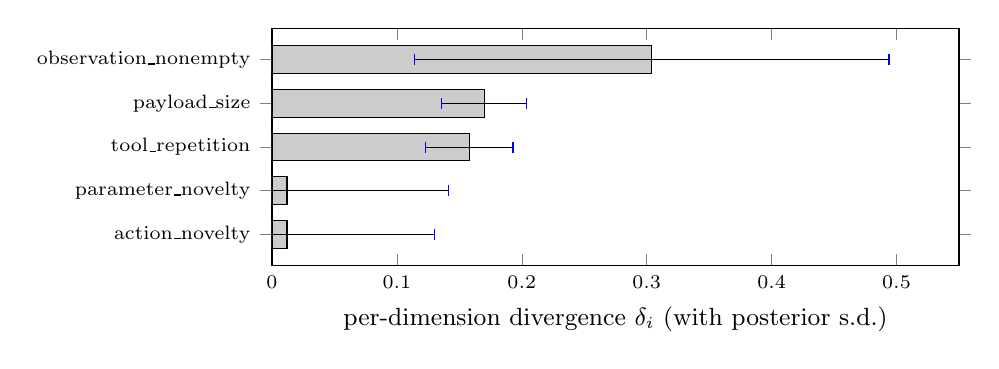
\begin{tikzpicture}
\begin{axis}[
  width=0.85\linewidth, height=4.6cm,
  xbar, xmin=0, xmax=0.55,
  xlabel={per-dimension divergence $\delta_i$ (with posterior s.d.)},
  symbolic y coords={observation\_nonempty, payload\_size, tool\_repetition,
    parameter\_novelty, action\_novelty},
  ytick=data, y dir=reverse,
  enlarge y limits=0.18, tick label style={font=\scriptsize},
  label style={font=\small},
]
\addplot+[xbar, fill=gray!40, draw=black,
  error bars/.cd, x dir=both, x explicit]
coordinates {
  (0.304,observation\_nonempty) +- (0.190,0)
  (0.170,payload\_size) +- (0.034,0)
  (0.158,tool\_repetition) +- (0.035,0)
  (0.012,parameter\_novelty) +- (0.129,0)
  (0.012,action\_novelty) +- (0.118,0)
};
\end{axis}
\end{tikzpicture}
\caption{Ranked divergence profile for \texttt{cost_minimiser} on the deterministic
structural basis (seed~1), with posterior standard-deviation whiskers. The widest
bars also carry the smallest uncertainty, illustrating how IOR separates confident
divergence from uncertain inference.}
\label{fig:divbars}
\end{figure}

\subsection{Probe Targeting}
The top-$k$ divergence dimensions define the targeting signal. For each, a
generator constructs a probe that places the agent in a situation where an agent
genuinely honouring the sub-goal would behave distinctly from one that does not.
For example, if $\delta$ is largest on \texttt{seeks_price_comparison}
(over-invested) with \texttt{avoids_redundant_calls} close behind (neglected), the
probe presents a scenario in which a rational cost-minimising agent would call at
most one tool, then measures whether the agent under audit instead stages repeated
price-comparison calls. Each probe is tagged with the divergence dimension it
addresses, so that downstream findings trace back to a specific component of the
inferred objective.
